\documentclass{book}
\usepackage[utf8]{inputenc}
\usepackage[ukrainian]{babel}
\usepackage{hyperref}
\usepackage{graphicx}

\title{Відкриті дані в Україні: посібник для початківців}
\author{Олександр Краковецький}
\date{2017}

\begin{document}

\maketitle

\tableofcontents

\chapter{Вступ}
\label{sec:introduction}

\textbf{Мета курсу} — ознайомити представників державних структур та громадського сектору (активістів, членів громадських організацій, журналістів тощо) з основними поняттями, принципами та підходами до роботи з даними. Курс допоможе підготувати та оприлюднити дані у форматах, що відповідають принципам відкритості та зручності обробки програмними засобами. Ви дізнаєтесь про переваги найбільш популярних форматів відкритих даних, міжнародну практику роботи з даними, а також особливості роботи з відкритими даними в Україні.

\begin{quote}
\textbf{Зверніть увагу:}\\
Ці методичні матеріали також будуть корисними для представників ІТ-сектору та бізнесу, які планують аналізувати публічні дані або працювати із суспільно-корисними ініціативами.
\end{quote}
\chapter{Про стан розвитку відкритих даних в Україні}

\textbf{За останні два роки Україна досягла великого прогресу в сфері відкритих даних, але все ще знаходиться досить далеко в міжнародних рейтингах.}

\subsection{Запущено єдиний державний портал відкритих даних data.gov.ua}

Перша версія порталу була розроблена волонтерами із організації Socialboost за підтримки міжнародних організацій і компанії Microsoft. На сьогоднішній день портал переданий на баланс Державного агентства з питань електронного урядування. На порталі доступно майже 6000 наборів даних від 700+ розпорядників, хоча якісних наборів даних у відсотковому співвідношенні не дуже багато.

\subsection{Запущено систему держваних закупівель ProZorro}

\href{https://prozorro.gov.ua}{ProZorro} – електронна система публічних закупівель яка прийшла на зміну паперовим держтендерам.

У Законі України «Про публічні закупівлі» передбачається:
\begin{itemize}
    \item Запровадження обов'язковості проведення процедур через електронну систему. (Перший етап — обов'язковість проведення процедур через електронну систему поширюється на головних розпорядників коштів та монополістів (з 1 квітня 2016 року), на другому (з 1 серпня) – на всіх замовників;
    \item Запровадження електронного аукціону, який передбачає автоматичну оцінку тендерних пропозицій;
    \item Визначення нових понять «авторизований електронний майданчик», «електронна система закупівель», «централізована закупівельна організація», «система хмарних обчислень»;
    \item Замість 5 процедур залишити 3 (відкриті торги, конкурентний діалог, переговорна процедура»;
    \item Зміна термінології, зокрема, замість терміну «державна закупівля» вводиться термін «публічна закупівля»; замість термінів «конкурс», «документація конкурсних торгів», «пропозиція конкурсних торгів», «комітет з конкурсних торгів», вводяться поняття «тендер», «тендерна документація», «тендерна пропозиція», «тендерний комітет».
\end{itemize}

ProZorro отримала міжнародну премію у сфері публічних закупівель Public Sector Procurement Award за створення і впровадження електронної системи з унікальною архітектурою. Розробка цієї системи на базі програмного забезпечення з відкритим кодом була здійснена у партнерстві влади, бізнесу та громадськості та адмініструвалася антикорупційною організацією \href{https://uk.wikipedia.org/wiki/%D0%A2%D1%80%D0%B0%D0%BD%D1%81%D0%BF%D0%B5%D1%80%D0%B5%D0%BD%D1%81%D1%96_%D0%86%D0%BD%D1%82%D0%B5%D1%80%D0%BD%D0%B5%D1%88%D0%BD}{Transparency International Україна}.

З 1 серпня 2016 року ProZorro є обов'язковою системою для всіх державних замовників при закупівлі від 200 тис. грн для товарів і від 1,5 млн грн для робіт.

\subsection{Запущено офіційний портал публічних фінансів України Є-Data}

Є-Data — це офіційний державний інформаційний портал у мережі Інтернет, на якому оприлюднюється інформація про використання публічних коштів та реалізується ідея «Прозорого бюджету». Задача - забезпечити повну прозорість державних фінансів та задовольнить право громадськості на доступ до інформації.

Основні законодавчі та нормативні засади для створення проекту:
\begin{itemize}
    \item \href{http://zakon3.rada.gov.ua/laws/show/183-19}{Закон України «Про відкритість використання публічних коштів»}
    \item План заходів з виконання Програми діяльності Кабінету Міністрів України та Стратегії сталого розвитку "Україна - 2020" у 2015 році п. 95: «Впровадження інтегрованої інформаційно-аналітичної системи "Прозорий бюджет" з метою забезпечення доступності інформації про державні фінанси для суспільних потреб із забезпеченням відкритої звітності за всіма коштами, використаними отримувачами бюджетних коштів..»
    \item Коаліційна угода Парламенту VIII скликання п. 2.5.10.: «Запровадження системи «Прозорий бюджет» з метою забезпечення доступності інформації про державні фінанси для суспільних потреб.
\end{itemize}

З 15 вересня 2015 року на порталі оприлюднюються всі трансакції Державної казначейської служби, з листопада на ньому доступна інформація про використання коштів державного і місцевих бюджетів, а у січні інформацію почали розкривати суб'єкти господарювання державної і комунальної власності, у статутному капіталі яких державна або комунальна частка акцій (часток, паїв) перевищує 50 відсотків.

До 2018 року планується забезпечити повний функціонал Інтегрованої інформаційно-аналітичної системи «Прозорий бюджет», яка своєю чергою торкнеться змін бюджетних процесів Міністерства фінансів, автоматизації систем ДФС та Казначейства, автоматизації систем обліку та звітності на місцевих рівнях.

\subsection{Запущено пошуково-аналітичну систему 007}

\href{https://www.facebook.com/pointOOSeven}{Пошуково-аналітична система 007} – це веб-сервіс на основі відкритих даних про використання публічних коштів. Проект передбачає сервіс пошуку та візуалізації даних з відкритих джерел про використання державою бюджетних коштів. Його ідея – дати громадськості інструмент контролю влади та можливість стежити за бюджетними витратами, збирати докази зловживань і швидко переводити боротьбу з корупцією в правове поле. Основний акцент зроблено на простоті використання та представлення специфічної інформації з масивів великих даних. Сайт був відкритий 8 квітня 2016 року.

\subsection{Нормативно-правове забезпечення}

9 квітня 2015 року Верховна Рада України ухвалила Закон України № 319 \href{http://zakon3.rada.gov.ua/laws/show/319-19}{«Про внесення змін до деяких законів України щодо доступу до публічної інформації у формі відкритих даних»}. Зазначеним Законом внесені зміни до Закону України «Про доступ до публічної інформації» з метою визначення базових норма та засад розвитку відкритих даних в Україні, а саме:

\begin{enumerate}
    \item Публічна інформація у формі відкритих даних - це публічна інформація у форматі, що дозволяє її автоматизоване оброблення електронними засобами, вільний та безоплатний доступ до неї, а також її подальше використання;
    \item Розпорядники інформації зобов'язані надавати публічну інформацію у формі відкритих даних на запит, оприлюднювати і регулярно оновлювати її на єдиному державному веб-порталі відкритих даних та на своїх веб-сайтах;
    \item Будь-яка особа може вільно копіювати, публікувати, поширювати, використовувати, у тому числі в комерційних цілях, у поєднанні з іншою інформацією або шляхом включення до складу власного продукту, публічну інформацію у формі відкритих даних з обов'язковим посиланням на джерело отримання такої інформації.
\end{enumerate}

21 жовтня 2015 року затверджено Постановою КМУ № 835 \href{http://zakon5.rada.gov.ua/laws/show/835-2015-%D0%BF}{«Про затвердження Положення про набори даних, які підлягають оприлюдненню у формі відкритих даних»}, якою визначено вимоги до формату і структури наборів даних, а також затверджено перелік пріоритетних наборів даних, які підлягають оприлюдненню (більше 300 наборів). Постановою чітко визначений перелік форматів для оприлюднення відкритих даних в залежності від їх виду:

\textbf{Текстові дані} \\
TXT, RTF, ODT, DOC(X), PDF (с текстовим змістом, скановане зображення), (X)HTML
21 жовтня 2015 року затверджено Постановою КМУ № 835 «[Про затвердження Положення про набори даних, які підлягають оприлюдненню у формі відкритих даних](http://zakon5.rada.gov.ua/laws/show/835-2015-%D0%BF)», якою визначено вимоги до формату і структури наборів даних, а також затверджено перелік пріоритетних наборів даних, які підлягають оприлюдненню (більше 300 наборів). Постановою чітко визначений перелік форматів для оприлюднення відкритих даних в залежності від їх виду:

**Текстові дані**  
TXT, RTF, ODT, DOC(X), PDF (с текстовим змістом, скановане зображення), (X)HTML

**Структуровані дані**  
RDF, XML, JSON, CSV, XLS(X), ODS, YAML

**Графічні дані**  
GIF, TIFF, JPG (JPEG), PNG

**Видеодані**  
MPEG, MKV, AVI, FLV, MKS, MK3D

**Аудіодані**  
MP3, WAV, MKA

**Дані, розроблені з використанням програми Macromedia Flash**  
SWF, FLV

**Архіви даних**  
ZIP, 7z, Gzip, Bzip2

Також, постановою передбачено, що державні реєстри, які постійно оновлюються, мають бути відкриті за допомогою API.

З метою забезпечення ефективного функціонування Єдиного державного веб-порталу відкритих даних та підвищення відкритості і прозорості діяльності органів виконавчої влади та місцевого самоврядування, Державним агентством з питань електронного урядування в лютому 2016 року розроблено проект постанови Кабінету Міністрів України «Деякі питання оприлюднення публічної інформації у формі відкритих даних», які знаходяться зараз на етапі обговорення. 

## Оцінка готовності України до розвитку відкритих даних

З метою визначення поточного стану розвитку та готовності України до розвитку відкритих даних, а також планування подальший дій, проведено оцінку готовності України до розвитку відкритих даних за методикою Всесвітнього банку ODRA.

Оцінка проводилась за восьма напрямами:

1. Зобов'язання Уряду;
2. Політичні і правові засади;
3. Інституційна структура, розподіл відповідальності та спроможність урядових структур;
4. Політика та процедури Уряду стосовно обробки даних;
5. Попит на відкриті дані;
6. Залучення громадського сектору та можливості для відкритих даних;
7. Фінансування політики відкритих даних;
8. Національна технологічна інфраструктура та навички.

Якщо коротко, з готовністю громадськості використовувати відкриті дані все добре, більш-менш хороша ситуація з готовністю уряду відкривати дані, технічною інфраструктурою, але все погано в плані фінансування, індустрією розробки продуктів на базі відкритих даних і захистом приватності. Детальний звіт знаходиться за [посиланням](http://dhrp.org.ua/uk/publikatsii1/1071-20160227-ua-publication) (є звіти на українській і англійській мовах).

## Дорожня карта розвитку відкритих даних

З метою забезпечення комплексного розвитку відкритих даних Державним агентством з питань електронного урядування напрацьовано Дорожню карту розвитку відкритих даних в Україні, яка містить 41 завдання по 5 напрямкам:

1. Підвищення доступності та якості відкритих даних;
2. Розвиток спроможності органів влади щодо публікації відкритих даних;
3. Посилення ролі відкритих даних в реалізації державної політики;
4. Нормативно-правове забезпечення;
5. Розвиток попиту та спроможності цільових аудиторій щодо використання відкритих даних.

Зазначений документ затверджено наказом Мінрегіону від 04.02.2016 року № 19. Повний текст розміщено за [посиланням](https://drive.google.com/file/d/0B1kGsKt9XV_QaFZVaTZiT19aRTA/view.).

## Хартія відкритих даних

Наразі Україною ініціюється приєднання до міжнародної Хартії відкритих даних.

Проект Постанови КМУ знаходиться за [посиланням](https://drive.google.com/file/d/0B1kGsKt9XV_QMEFNNklzRXdaSDA/view?usp=sharing).

Розробка Міжнародної хартії була ініційована представниками урядів Канади, Мексики, Великобританії, впливових міжнародних організацій у травні 2015 року під час міжнародної конференції з питань відкритих даних у Канаді.

Головною метою Міжнародної Хартії відкритих даних є покращення та сприяння співпраці та взаємоузгодженості для прийняття та реалізації спільних принципів, стандартів та кращих практик відкритих даних по всьому світу. Цілями Хартії є поширення демократії, боротьба з корупцією та сприяння економічному зростанню по всьому світу. Хартія визначає 6 головних принципів та шляхи розвитку відкритих даних для країни.

## Світові та українські компетенції й рейтинги

Сьогодні найбільш важливими є наступні два рейтинги оцінювання стану розвитку відкритих даних:

1. [Open Data Barometer](http://opendatabarometer.org/data-explorer/?_year=2015&indicator=ODB&open=UKR). За цим рейтингом Україна посідає 62 місце.

2. [Open Data Index](http://index.okfn.org/place/ukraine). За цим рейтингом Україна посідає 54 місце (із 122).

Україна співпрацює з такими міжнародними організаціями в сфері відкритих даних: 

1. [Open Data Institute](http://theodi.org). Займається розвитком відкритих даних по всьому світу, формуванням стандартів та єдиних підходів, розвитком компетенцій.

2. [Open knowledge foundation](https://okfn.org). Займається підтримкою громадських інституцій щодо розвитку відкритих даних, а також розвитком відкритої платформи для побудови порталів відкритих даних CKAN.

3. [Open Data for Development](http://od4d.net). Займається підтримкою ініціатив з розвитку відкритих даних по всьому світу, а також організацію міжнародної співпраці.

В останньому рейтингу E-Government Development Index (EGDI) 2016 Україна зайняла 62 місце серед 193 країн, покращивши свою позицію на 25 пунктів.

## Професійні українські організації і ініціативи

В Україні запущений інкубатор відкритих даних 1991, який системно займається відбором проектів, їх інкубацією і пошуком інвестицій. На сьогодні уже було два набори в інкубаційну програму. 

На початку року розпочався EGAP Challenge – конкурс ІТ проектів в області електронної демократії, соціальної сфери і проектів в сфері відкритих даних. Спільна ініціатива Державного агентства з питань електронного урядування, Фонду Східної Європи в рамках реалізації Програми EGAP, що фінансується Швейцарською Конфедерацією, має на меті не тільки запровадити нові інструменти e-democracy в чотирьох регіонах України (Вінницький, Волинській, Дніпровській та Одеській областях), а також показати українським стартапам нову нішу, в якій можливо створювати якісні проекти, що мають змогу безпосередньо впливати на місцеву і центральну влади. А влада – у свою чергу – отримає набір нових інструментів для росту ефективності її роботи і прозорості взаємодії з платниками податків.

Пріоритетними є напрямки:

* створення нових інструментів взаємодії влади і суспільства, особливо в частині надання можливості громадянам напряму впливати на процеси прийняття управлінських рішень;

* підвищення прозорості і відкритості діяльності органів влади, особливо в частині формування і виконання бюджетів, надання дозвільних документів і тому подібне;

* створення нових якісних сервісів для громадян і бізнесу, особливо в частині надання публічних послуг;

* розвиток проектів на базі відкритих даних;

* вирішення соціальних проблем;

* об'єднання і налагодження ефективного співробітництва громадян для вирішення загальних проблем;

* проекти в області Smart City;

* галузеві проекти, спрямовані на підвищення ефективності державного управління і обслуговування громадян та бізнесу (е-екологія, е-медицина, е-освіта і т.д.).

В чотирьох областях пройшли креативні уікенди на яких було відібрано 15 проектів для проходження двомісячної інкубації. Партнерами конкурсу виступили компанії Cisco, IBM, DeNovo, Intel.

В Україні діють потужні громадські організації, що працюють з відритими даними— ОПОРА, Чесно, Канцелярська сотня, Vox Ukraine і інші. Результат — десятки досліджень, проекти по візуалізації даних, моніторинг відкритих наборів даних, десятки заходів по усій країні. Декілька проектів уже імплементовані в державні служби і проекти "смарт сіті". 

Наприклад, відкриті дані Укрзалізниці дали можливість провести масштабне дослідження – хто куди подорожує, які ключові станції, як розподіляється потік пасажирів і інші візуалізації.

## Рекомендації по роботі з відкритими даними

На сайті Верховної Ради є [інструкція](http://data.rada.gov.ua/open/main/opendata) по роботі з відкритими даними.

Також спільно з Агентством з питань електронного врядування та ПРООН були розроблені [методичні рекомендації щодо оприлюднення наборів даних у формі відкритих даних](https://drive.google.com/file/d/0B1kGsKt9XV_QWjhaZ0ZMVmFiUE0/view).

Метою рекомендацій є ознайомлення відповідальних осіб розпорядників інформації з ключовими питаннями, що постають у процесі оприлюднення наборів даних у формі відкритих даних. Також, методичні рекомендації будуть корисні розробникам застосунків на базі відкритих даних, громадським організаціям, засобам масової інформації та громадянам, які мають намір працювати з відкритими даними.

Проект першої версії Методичних рекомендацій підготовлено на основі найбільш популярних загальних запитань від розпорядників інформації, але, безумовно, ще не охоплює усіх піднятих розпорядниками інформації та громадськістю питань. Методичні рекомендації будуть систематично оновлюватися з метою забезпечення розпорядників інформації необхідною інформацією для оприлюднення наборів даних.

---

В цілому, Україна знаходиться лише на початку з точки зору відкритості державних служб, створення інститутів моніторингу діяльності депутатів, чиновників і міських служб, дигіталізації державних послуг. За наявності політичної волі, допомоги міжнародних організацій, а також за умови координації громадських організацій, бізнесу та ІТ сектору Україна здатна на досить короткий термін значно поліпшити свої показники в області електронного врядування та відкритих даних.

\chapter{Що таке відкриті дані?}

\subsection{Визначення відкритих даних}

\textbf{Відкриті дані (англ. Open Data)} – це концепція, яка відображає ідею, що визначені дані мають бути доступні для легкої обробки програмними засобами (machine readable) та подальшого використання і розповсюдження без жодних обмежень і контролю, в тому числі й для комерційного використання. Відкриті дані – це не просто інформація, а концепція, тобто система поглядів, підходів, процесів, які мають одну ідею та мету – вільного використання і розповсюдження даних про діяльність державних органів та органів місцевого самоврядування через мережу Інтернет.

Згідно загальноприйнятої в світі концепції, обов’язково безоплатними можуть бути тільки ті дані, які знаходяться у власності держави («ліцензійно чисті»), і якщо вони подаються в первинному необробленому вигляді. Додаткова обробка або доступ до API частіше за все лімітуються або коштують грошей. Крім того, хто завгодно може (з обов’язковим посиланням на джерело) використати дані в комерційний спосіб, створити на базі них власну програму чи обробити та надати нову цінність (розкласифікувати, встановити зв’язки тощо). Безумовно, всі витрати на додаткову роботу редакторів, програмістів та інше оплачує замовник (або кінцевий користувач).

Відкриті дані дозволяють повторно і необмежено використовувати інформацію, поєднувати її між собою, зменшити або виключити зайві витрати на дублювання та опрацювання великих масивів даних, реєстрів, довідників, баз даних тощо, створених в різних органах влади.

Закон "Про внесення змін до деяких законів України щодо доступу до публічної інформації у формі відкритих даних" №2171 від 19.02.2015 (прийнятий 09.04.2015) визначає наступний термін:

\begin{quote}
\textbf{Публічна інформація у формі відкритих даних} – це публічна інформація у форматі, що дозволяє її автоматизоване оброблення електронними засобами, вільний та безоплатний доступ до неї, а також її подальше використання.
\end{quote}

\subsection{Класифікація відкритих даних}

В законопроекті одночасно використовуються поняття «форма» та «формат», що не є тотожними. Розглянемо детально.

Для того, щоб зрозуміти, які можуть бути форми відкритих даних, ми також звернемося до відомої класифікації \textbf{«5 зірок Open Data»} (\url{http://5stardata.info/}), де якість даних та рівень відкритості визначається кількістю зірок від 1 до 5, чим більше – тим краще. Відкритість даних залежить від способів доступу, форматів та кількості додаткових дій, які потрібні для отримання кінцевої інформації, її обробки та збереження у власному сховищі або базі даних.

\begin{figure}[h]
    \centering
    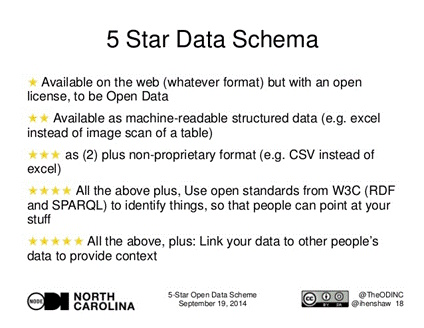
\includegraphics[width=\textwidth]{images/001.gif}
    \caption{5 зірок Open Data}
\end{figure}

\begin{itemize}
    \item \textbf{Одну зірку (*)} отримує будь-яка інформація, вільно доступна через Інтернет в будь-якому форматі. Під цю класифікацію підпадає файл у форматі PDF або інша (сканована) копія документу, на який веде пряме посилання на офіційному сайті державного органу.
    \item \textbf{Дві зірки (**)} отримує структурована інформація, яку можна обробляти автоматично, наприклад, у форматах для веб-браузерів чи офісних програм (відкриті формати – TXT, HTML, RSS; пропрієтарні формати, Excel – XLS, Word – DOC, RTF).
    \item \textbf{Три зірки (***)} може отримати інформація, представлена у відомих, добре описаних відкритих структурованих форматах (наприклад, CSV, JSON, XML, YAML).
    \item \textbf{Чотири зірки (****)} надаються у випадку, якщо можна отримати первинні необроблені набори відкритих даних у вигляді файлів або фільтровані дані у запиті до API за вказаними параметрами.
    \item \textbf{П’ять зірок (*****)} надається інформації, коли набори відкритих даних пов’язані між собою і представляють собою семантичну мережу.
\end{itemize}

\subsection{Формати даних}

В залежності від специфіки даних, їх розміру та тематики (геологія, тендери, реєстри, судові документи тощо), одні проекти відкритих даних створювались на базі наборів PDF чи DOC файлів, таблиць XLS, що перетворювались на прості текстові таблиці CSV, а інші брали за основу формат розмітки XML, проектували власні схеми XSD і використовували складні структури.

\subsubsection{Табличні формати}

\paragraph{CSV (Comma-Separated Values)}

CSV (від англ. \textit{Comma-Separated Values} – значення, що розділені комами) – текстовий відкритий формат, призначений для представлення таблиць (масивів, наборів) даних.

\begin{verbatim}
1997,Ford,E350,"ac, abs, moon",3000.00  
1999,Chevy,"Venture ""Extended Edition""","",4900.00  
1996,Jeep,Grand Cherokee,"MUST SELL! air, moon roof, loaded",4799.00  
\end{verbatim}

\paragraph{XLS/XLSX (Document Office Open XML)}

Файл XLSX - електронна таблиця, створена в Microsoft Excel - додатку для роботи з таблицями.

\subsubsection{Графічні формати}

\paragraph{JPEG (Joint Photographic Experts Group)}

JPEG (англ. \textit{Joint Photographic Experts Group}) - один з популярних графічних форматів, застосовуваний для зберігання фотозображень.

\paragraph{PNG (Portable Network Graphics)}

PNG (англ. \textit{Portable network graphics}) - растровий формат зберігання графічної інформації, що використовує стиснення без втрат.

\paragraph{TIFF (Tagged Image File Format)}

TIFF (англ. \textit{Tagged Image File Format}) - формат зберігання растрових графічних зображень.

\subsubsection{Текстові формати}

\paragraph{TXT (Textfile)}

TXT - це формат, що містить текстові дані, які, як правило, організовані у вигляді рядків.

\paragraph{Markdown}

Markdown - полегшена мова розмітки, створена з метою написання максимально читабельного і зручного для редагування тексту.

\subsubsection{Текстово-графічні формати}

\paragraph{HTML (HyperText Markup Language)}

HTML (від англ. \textit{HyperText Markup Language}) - стандартна мова розмітки документів у Всесвітній павутині.

\paragraph{DOCX (Document Office Open XML)}

DOCX (\textit{Document Office Open XML}) - формат файлу для зберігання електронних документів пакетів офісних додатків.

\paragraph{OpenDocument format (LibreOffice/OpenOffice)}

Формат OpenDocument - це формат для текстових, табличних документів та презентацій.

\paragraph{PDF (Portable Document Format)}

Формат переносного документа (PDF) - це формат файлу, який використовується для надійного уявлення і обміну документами.

\subsubsection{Формати представлення даних через API}

\paragraph{JSON (JavaScript Object Notation)}

JSON (від англ. \textit{JavaScript Object Notation}) – текстовий відкритий формат, оснований на Javascript представлені.

\begin{verbatim}
{
    "firstName": "Иван",
    "lastName": "Иванов",
    "address": {
        "streetAddress": "Московское ш., 101, кв.101",
        "city": "Ленинград",
        "postalCode": 101101
    },
    "phoneNumbers": [
        "812 123-1234",
        "916 123-4567"
    ]
}
\end{verbatim}

\paragraph{XML (eXtensible Markup Language)}

XML (від англ. \textit{eXtensible Markup Language}) – мова розмітки, що розширюється.

\begin{verbatim}
<person firstName="Иван" lastName="Иванов">
    <address streetAddress="Московское ш., 101, кв.101"
        city="Ленинград" postalCode="101101"/>
    <phoneNumbers>
        <phoneNumber>812 123-1234</phoneNumber>
        <phoneNumber>916 123-4567</phoneNumber>
    </phoneNumbers>
</person>
\end{verbatim}

\subsubsection{Формати даних для роботи з геопросторовими даними}

\paragraph{GeoJSON та TopoJSON}

GeoJSON - відкритий формат, призначений для зберігання графічних структур даних.

\begin{verbatim}
{
    "type": "FeatureCollection",
    "features": [
        {
            "type": "Feature",
            "geometry": {"type": "Point", "coordinates": [102.0, 0.5]},
            "properties": {"prop0": "value0"}
        },
        {
            "type": "Feature",
            "geometry": {
                "type": "LineString",
                "coordinates": [
                    [102.0, 0.0], [103.0, 1.0], [104.0, 0.0], [105.0, 1.0]
                ]
            },
            "properties": {
                "prop0": "value0",
                "prop1": 0.0
            }
        },
        {
            "type": "Feature",
            "geometry": {
                "type": "Polygon",
                "coordinates": [
                    [ [100.0, 0.0], [101.0, 0.0], [101.0, 1.0],
                        [100.0, 1.0], [100.0, 0.0] ]
                ]
            },
            "properties": {
                "prop0": "value0",
                "prop1": {"this": "that"}
            }
        }
    ]
}
\end{verbatim}

\chapter{Публікація та оновлення відкритих даних}

\subsection{Вибір формату даних та конвертація даних з одного формату в інший}

Вибір формату даних залежить від способу збереження та інших факторів, проте в більшості випадків можна користуватись такими загальними правилами:

\begin{enumerate}
    \item \textbf{Неструктуровані текстові дані} (тексти законів, розпоряджень, довідкових даних):  
        \begin{itemize}
            \item Найкращий формат — Markdown або TXT.  
            \item Markdown підтримує додаткову розмітку (заголовки, абзаци, посилання, зображення тощо).  
            \item Вказуйте різновид Markdown.  
            \item HTML — гірший варіант, doc/docx, pdf/tiff — найгірші (окрім випадків, коли потрібна копія оригінального документу із підписом та печаткою).
        \end{itemize}
    \item \textbf{Табличні дані:}  
        \begin{itemize}
            \item Використовуйте формат CSV, у гіршому випадку — XLS/XLSX.
        \end{itemize}
    \item \textbf{Скани документів:}  
        \begin{itemize}
            \item Найкращий формат — TIFF, потім — PDF.
        \end{itemize}
    \item \textbf{Зображення:}  
        \begin{itemize}
            \item Обов'язкова роздільна здатність для OCR — не менше 300 dpi.
        \end{itemize}
    \item \textbf{Великі файли або групи файлів:}  
        \begin{itemize}
            \item Архівуйте у форматі ZIP/7Z.  
            \item Для файлів понад 4 ГБ — RAR.
        \end{itemize}
    \item \textbf{Дані, що змінюються постійно і формуються «на льоту»:}  
        \begin{itemize}
            \item Не обов'язково зберігати у вигляді файлів.  
            \item Достатньо надати доступ через Інтернет-адреси або API.  
            \item Рекомендовані формати для API: JSON/XML/RDF.
        \end{itemize}
    \item \textbf{Бінарні формати:}  
        \begin{itemize}
            \item Використовуйте лише за відсутності альтернативи.
        \end{itemize}
\end{enumerate}

Для конвертації даних існує багато інструментів: онлайн-сервіси, програмні засоби, бібліотеки. Зазвичай немає проблем з конвертацією між відкритими форматами. Проблеми можуть виникати з Word/PDF.

\textbf{Деякі програмні засоби для конвертації:}

\begin{itemize}
    \item Microsoft Word, Excel, Access
    \item Графічні формати та PDF: Adobe Photoshop, Acrobat Reader, Foxit PDF Reader, Paint.NET, Corel Draw
    \item Текстові дані: Notepad++
    \item Програмні засоби: SPSS, Microsoft Azure ML, Matlab
    \item Онлайн інструменти:  
        \begin{itemize}
            \item \href{http://konklone.io/json/}{JSON to CSV}  
            \item \href{http://www.convertcsv.com/csv-to-json.htm}{CSV to JSON}  
            \item \href{http://json2csharp.com/}{JSON to C\#}
        \end{itemize}
    \item Очищення HTML документів від Word-стилів: \href{https://word2cleanhtml.com/}{word2cleanhtml.com}
\end{itemize}

\subsection{Основні помилки при оприлюдненні відкритих даних}

\subsubsection{Чому Excel формат не є рекомендованим форматом?}

В Постанові дозволяється використовувати XLS/XLSX (Microsoft Excel). Проте Excel дозволяє додавати розширене форматування, об’єднані комірки, вбудовані об’єкти, макроси та формули, що ускладнює машинну обробку.

\textbf{Приклади неправильних Excel-документів:}

\begin{figure}[h]
    \centering
    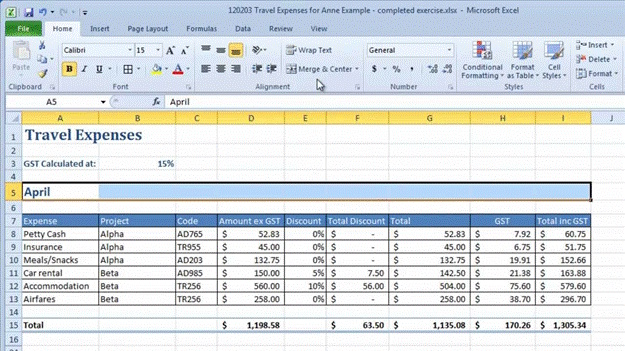
\includegraphics[width=0.5\textwidth]{images/004.gif}
    \caption{Неправильний Excel 1}
\end{figure}

\begin{figure}[h]
    \centering
    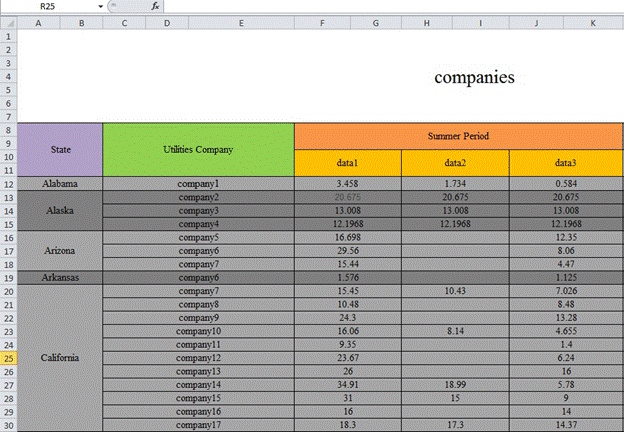
\includegraphics[width=0.5\textwidth]{images/005.gif}
    \caption{Неправильний Excel 2}
\end{figure}

\textbf{Приклади правильних Excel-файлів:}

\begin{figure}[h]
    \centering
    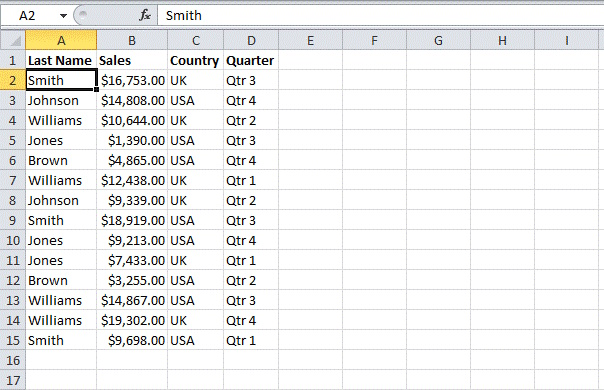
\includegraphics[width=0.5\textwidth]{images/006.gif}
    \caption{Правильний Excel 1}
\end{figure}

\begin{figure}[h]
    \centering
    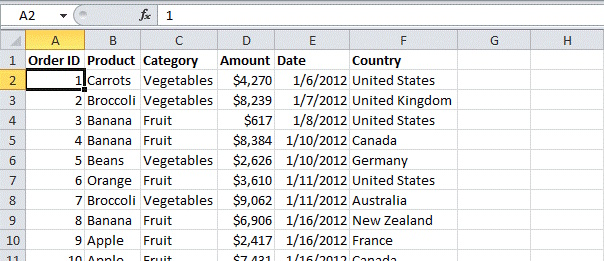
\includegraphics[width=0.5\textwidth]{images/007.gif}
    \caption{Правильний Excel 2}
\end{figure}

Дані у правильному форматі легко експортувати у CSV.

\subsubsection{Оприлюднення занадто агрегованих даних}

\textbf{Очікується:}  
\begin{itemize}
    \item ділянка та її координати  
    \item дата ДТП  
    \item кількість постраждалих та тип ушкоджень  
    \item область (місто)  
    \item стан ділянки
\end{itemize}

\textbf{Неправильно:}  
\begin{itemize}
    \item лише кількість ДТП по областях
\end{itemize}

Розпорядники повинні публікувати детальну інформацію на рівні транзакцій, випадків або подій.

\subsection{Призначення відповідальних за розкриття даних}

Кожен розпорядник повинен визначити відповідальних осіб за аудит, обробку та публікацію відкритих даних. Вони повинні знати про доступні набори, формати, розміри, роботу з базами даних та користуватись порталом відкритих даних.

\subsection{Аудит наборів відкритих даних і пріоритетність їх публікації}

Публікація даних здійснюється поетапно, враховуючи:

\begin{enumerate}
    \item Потребу споживачів (за методикою моніторингу)
    \item Ступінь готовності (наявність даних, технічна готовність)
    \item Витрати на публікацію та підтримку
\end{enumerate}

\textbf{Фактори для формування реєстру:}

\begin{itemize}
    \item Публікуються дані без попередньої обробки
    \item Визначена відповідальна особа за кожен набір
    \item Встановлена періодичність оновлення
\end{itemize}

Реєстр затверджується органом і публікується на офіційному сайті.

\subsection{Підготовка даних до публікації}

\subsubsection{Кодування файлів}

Текст зберігається у вигляді числових значень згідно стандарту кодування.

\begin{itemize}
    \item \textbf{Windows-1251} — стандартне кодування для українських і російських версій Windows.  
        \href{https://uk.wikipedia.org/wiki/Windows-1251}{Детальніше}
    \item \textbf{UTF-8} — універсальне кодування, сумісне з ASCII.  
        \href{https://uk.wikipedia.org/wiki/UTF-8}{Детальніше}
\end{itemize}

Більшість державних органів використовують Windows-1251, що несумісне з іншими ОС. Перед публікацією на data.gov.ua переконайтесь, що файли збережені у UTF-8.

\textbf{Приклад проблем з кодуванням:}

\begin{figure}[h]
    \centering
    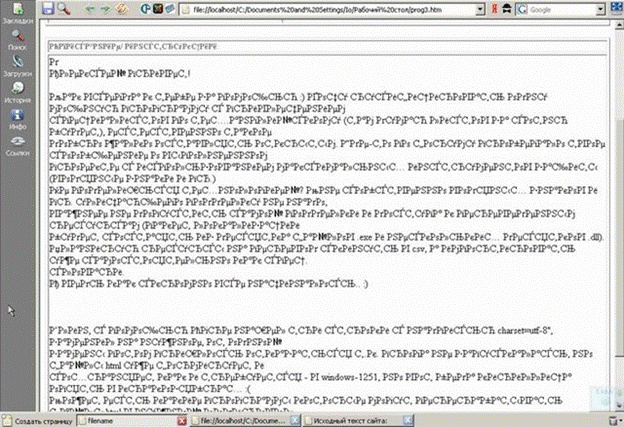
\includegraphics[width=0.5\textwidth]{images/008.gif}
    \caption{Проблеми з кодуванням}
\end{figure}

\subsubsection{Один файл чи декілька?}

Якщо дані — реляційна база (MySQL, SQL Server, Oracle):

\begin{figure}[h]
    \centering
    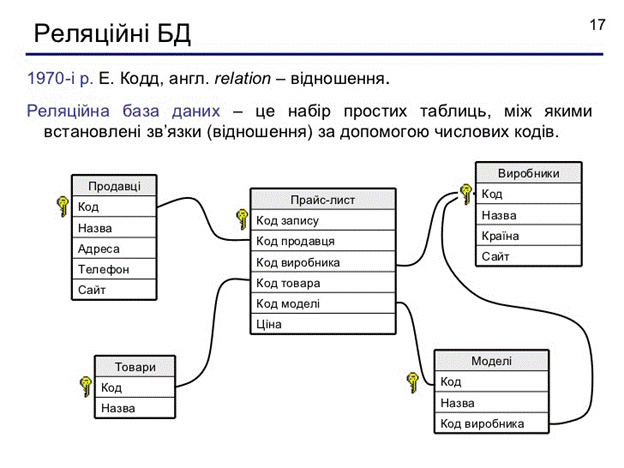
\includegraphics[width=0.5\textwidth]{images/009.gif}
    \caption{Схема бази}
\end{figure}

\textbf{Приклад:}

\textit{Vendors (виробники)}

\begin{tabular}{|c|c|c|c|}
\hline
Id & Name      & Country & Website              \\
\hline
1  & Microsoft & USA     & http://microsoft.com \\
2  & Apple     & USA     & http://apple.com     \\
\hline
\end{tabular}

\textit{Models (моделі)}

\begin{tabular}{|c|c|c|}
\hline
Id & Name    & Vendor Code \\
\hline
1  & Surface & 1           \\
2  & iPhone  & 2           \\
\hline
\end{tabular}

\textbf{Варіант 1: Один файл}

\begin{verbatim}
models.csv:
Id;Name;Vendor;Country;Website
1;Surface;Microsoft;USA;http://microsoft.com
2;iPhone;Apple;USA;http://apple.com
\end{verbatim}

\textbf{Варіант 2: Два файли}

\begin{verbatim}
vendors.csv:
Id;Name;Country;Website
1;Microsoft;USA;http://microsoft.com
2;Apple;USA;http://apple.com

models.csv:
Id;Name;VendorId
1;Surface;1
2;iPhone;2
\end{verbatim}

\textbf{Порівняння:}

\begin{tabular}{|l|l|l|}
\hline
Критерій                           & Один файл                                                & Багато файлів                        \\
\hline
Збитковість даних                   & Велика                                                  & Мала                                 \\
Фінальний розмір                    & Більший                                                 & Менший                               \\
Перевірка на цілісність             & Складна                                                 & Проста                               \\
Готовність до використання через API & Погана                                                  & Хороша                               \\
Кількість запитів                   & Один (перевага для малих файлів)                        & Багато                               \\
\hline
\end{tabular}

Другий варіант доцільніший.

\subsubsection{Деперсоніфікація даних}

Згідно \href{http://zakon3.rada.gov.ua/laws/show/2297-17}{Закону “Про захист персональних даних”}, персональні дані — будь-які відомості, за якими ідентифікується особа. Такі дані мають бути деперсоніфіковані перед публікацією.

\textbf{Приклад:}

\textit{Початкові дані:}

\begin{tabular}{|l|l|l|l|}
\hline
ПІП         & Місто & Телефон      & Група крові \\
\hline
Іванов І.І. & Київ  & 011 111 11 11& A(I)+       \\
Петров П.П. & Одеса & 011 111 11 12& B(II)-      \\
\hline
\end{tabular}

\textit{Кроводачі:}

\begin{tabular}{|l|l|l|}
\hline
ПІП         & Центр    & Дата       \\
\hline
Іванов І.І. & Охматдит & 01.01.2016 \\
Петров П.П. & Охматдит & 01.02.2016 \\
\hline
\end{tabular}

\textit{Після деперсоніфікації:}

\begin{tabular}{|l|l|l|}
\hline
ПІП & Місто & Група крові \\
\hline
1   & Київ  & A(I)+       \\
2   & Одеса & B(II)-      \\
\hline
\end{tabular}

\textit{Кроводачі:}

\begin{tabular}{|l|l|l|}
\hline
ПІП & Центр    & Дата       \\
\hline
1   & Охматдит & 01.01.2016 \\
2   & Охматдит & 01.02.2016 \\
\hline
\end{tabular}

\subsubsection{Архівація наборів даних}

Архівація зменшує розмір файлів і трафік. Текстові дані стискаються до 90\%, Word/Excel/PDF — на 10-60\%, зображення — майже не стискаються.

\textbf{Архівувати потрібно:}

\begin{itemize}
    \item історичні дані
    \item файли понад 50 МБ
    \item застарілі версії наборів
    \item багатотомні набори
\end{itemize}

\textbf{Рекомендовані формати:} zip/7z/tar.  
\textbf{Рекомендована програма:} \href{http://7-zip.org.ua/}{7-zip}

\subsubsection{Публікація даних, що мають періодичність}

Набори поділяються на:

\begin{itemize}
    \item \textbf{Частопубліковані} (оновлення частіше 1 раз на тиждень)
    \item \textbf{Рідкопубліковані} (рідше 1 раз на тиждень)
\end{itemize}

В паспорті набору вказується дата останнього оновлення.

\textbf{Частота оновлень:}

\begin{itemize}
    \item Часто: більше одного разу в день, щодня, щотижня
    \item Рідко: щомісяця, щокварталу, кожні півроку, щороку, по мірі змін
\end{itemize}

\textbf{Приклади іменування файлів:}

\begin{itemize}
    \item За датою: \texttt{exchange\_20160101.csv}
    \item За валютою: \texttt{exchange\_usd.csv}
\end{itemize}

Якщо дані змінюються постійно — організуйте доступ через API.

\subsubsection{Публікація схожих даних з різними структурами}

Якщо структура схожа — об'єднайте всі поля, відсутні дані залишайте порожніми.

\textbf{Приклад:}

\begin{verbatim}
A1,A2,A3,A4
1,1,1,1

A1,A2,A3,A5
2,2,2,2
\end{verbatim}

\textbf{Фінальний файл:}

\begin{verbatim}
A1,A2,A3,A4,A5
1,1,1,1,
2,2,2,,2
\end{verbatim}

Якщо структура відрізняється значно — розглядайте файли окремо.

\subsubsection{Публікація даних у вигляді API та робота з великими обсягами}

Два основних способи доступу:

\begin{itemize}
    \item \textbf{Data Hub} — для рідко змінюваних даних
    \item \textbf{API} — для оперативних запитів
\end{itemize}

Рекомендується використовувати \href{http://www.odata.org/}{OData} для API.

В описі набору вказуйте тип даних, посилання на документацію, умови доступу, обмеження, формати, підтримку OData.

\subsubsection{Канали розповсюдження відкритих даних}

\begin{enumerate}
    \item Через сайт \href{https://data.gov.ua}{data.gov.ua}
    \item Через сайти місцевих органів самоврядування
    \item За допомогою API
    \item Через ftp-сервер
    \item Через BitTorrent
\end{enumerate}

\chapter{Відкриті дані в Україні}

\section{Законодавство України щодо відкритих даних та готовність країни до впровадження}

\begin{enumerate}
    \item \href{http://zakon2.rada.gov.ua/laws/show/319-19}{Положення про набори даних, які підлягають оприлюдненню у формі відкритих даних № 835 (редакція від 21.10.2015)}
    \item \href{https://drive.google.com/file/d/0B1kGsKt9XV_QaFZVaTZiT19aRTA/view}{План заходів (дорожня карта) розвитку відкритих даних на 2016 рік}
    \item Єдиний державний портал відкритих даних \href{https://data.gov.ua/}{data.gov.ua — Керівництво користувача}
    \item Єдиний державний портал відкритих даних \href{https://data.gov.ua/}{data.gov.ua — Робота з API}
    \item \href{https://docs.google.com/document/d/1g5VUhUzjgTVvcp7zvlWbCUsmoJNaQ6w4T3vacYSu34U/edit}{Open Data Readiness Assessment (ODRA) Ukraine Final Report}
\end{enumerate}

\section{Україна у світових рейтингах}

\subsection{Open Data Barometer}

\begin{itemize}
    \item Сайт: \href{http://www.opendataresearch.org/barometer}{opendataresearch.org/barometer}
\end{itemize}

Open Data Barometer — спільний дослідницький проєкт Open Data Institute та World Wide Web Foundation. Аналізує глобальні тенденції розвитку відкритих даних, надає порівняльні дані по країнах і регіонах. Україна займає 62 місце із 86 проаналізованих країн (2015 — 55 місце).

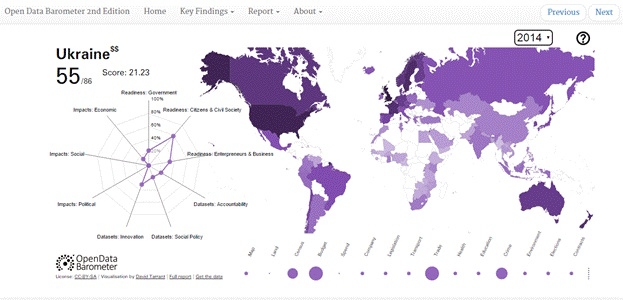
\includegraphics{images/010.jpg}
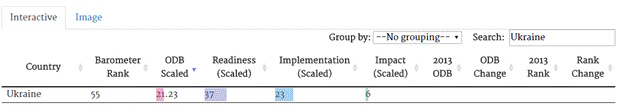
\includegraphics{images/011.jpg}
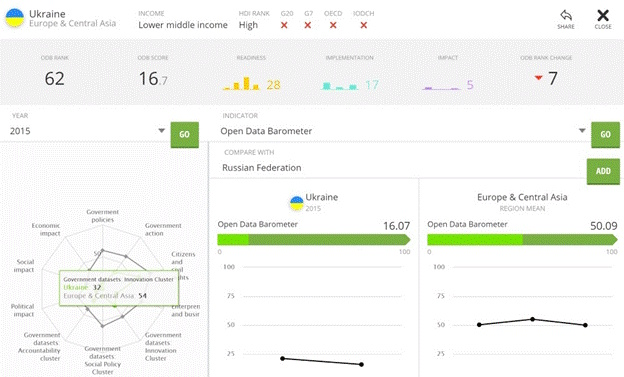
\includegraphics{images/012.jpg}

\subsection{Open Data Index}

\begin{itemize}
    \item Сайт: \href{https://index.okfn.org/}{index.okfn.org}
\end{itemize}

Масштабний дослідницький проєкт Open Knowledge Foundation щодо відкритості державних даних у світі. Україна — 54 місце у глобальному рейтингу (2015 рік).

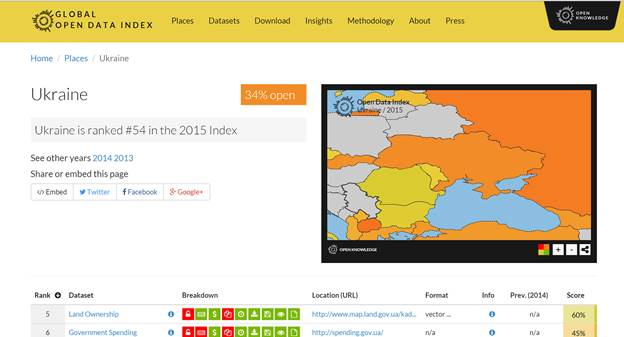
\includegraphics{images/013.jpg}

\subsection{The Web Index}

\begin{itemize}
    \item Сайт: \href{http://thewebindex.org/}{thewebindex.org}
\end{itemize}

Рейтинг розвитку інтернету в країнах світу від World Wide Web Foundation. Україна — 46 місце серед 86 країн.

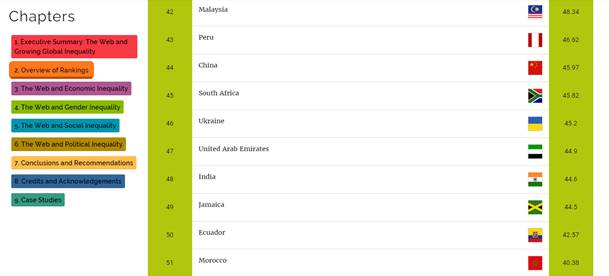
\includegraphics{images/014.jpg}

\subsection{Open Budget Survey}

\begin{itemize}
    \item Сайт: \href{http://internationalbudget.org/what-we-do/open-budget-survey/}{internationalbudget.org/what-we-do/open-budget-survey/}
\end{itemize}

Рейтинг відкритості державних бюджетів від International Budget Partnership. Оцінки для України:
\begin{itemize}
    \item Прозорість (відкритий бюджет): 46/100
    \item Участь громадськості: 23/100
    \item Нагляд державним органом: 79/100
    \item Нагляд вищого органу фінансового контролю: 83/100
\end{itemize}

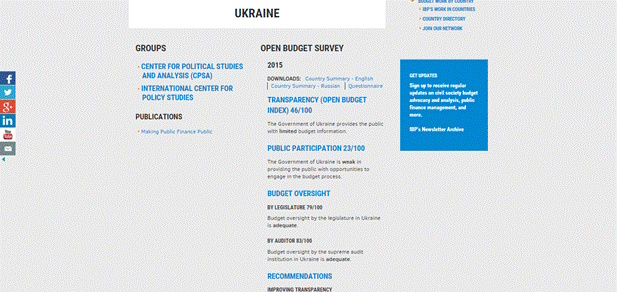
\includegraphics{images/015.jpg}

\subsection{E-Government for the People}

\begin{itemize}
    \item Сайт: \href{http://www.unpan.org/egovkb/global_reports/08report.html}{unpan.org/egovkb/global_reports/08report.html}
\end{itemize}

Рейтинг ООН з розвитку електронного уряду. Коефіцієнт розвитку електронного уряду України — між 0,5 та 0,75.

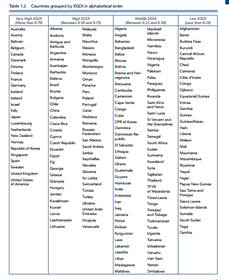
\includegraphics{images/016.jpg}

\section{Проєкти на базі відкритих даних}

\subsection{Нові назви вулиць, площ Дніпропетровська}

\begin{itemize}
    \item \href{http://rename.dp.ua/}{rename.dp.ua} — повний перелік нових назв вулиць і площ Дніпропетровська.
\end{itemize}

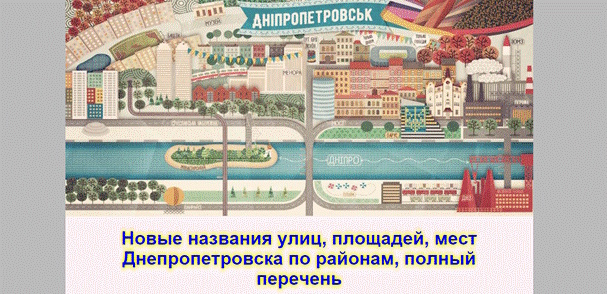
\includegraphics{images/017.jpg}

\subsection{ДонорUA}

\begin{itemize}
    \item \href{http://donor.ua/}{donor.ua} — координація донорів крові та пропаганда донорства в Україні.
\end{itemize}

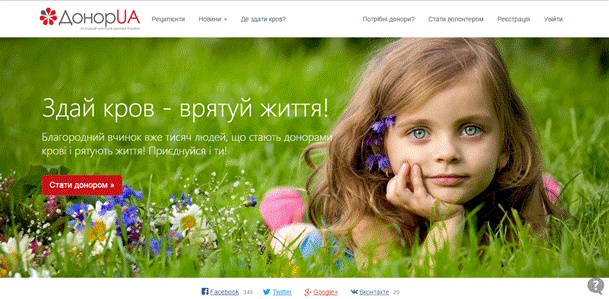
\includegraphics{images/018.jpg}

\subsection{УкрТрансГаз}

\begin{itemize}
    \item \href{http://utg.ua/live/}{utg.ua/live/} — карта трубопроводів, сховищ та обсягів газу.
\end{itemize}

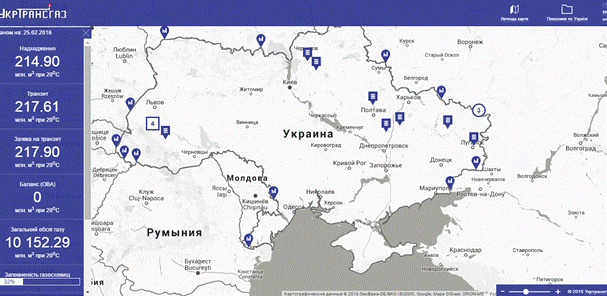
\includegraphics{images/019.jpg}

\subsection{НБУ}

\begin{itemize}
    \item \href{http://nbu.rocks/}{nbu.rocks} — відкриті дані Національного Банку України про банки.
\end{itemize}

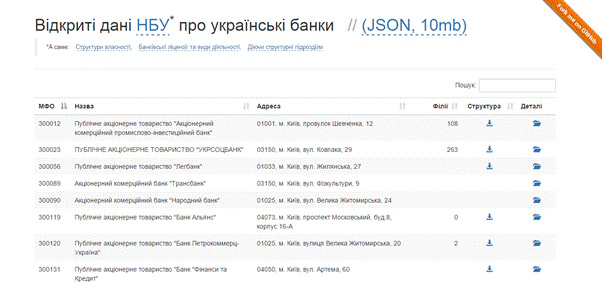
\includegraphics{images/020.jpg}

\subsection{3G.Multitest.ua}

\begin{itemize}
    \item \href{http://3g.multitest.ua/}{3g.multitest.ua} — карта покриття 3G GSM операторів України.
\end{itemize}

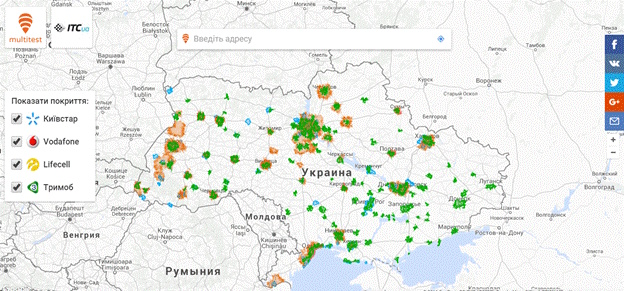
\includegraphics{images/021.jpg}

\subsection{Агенти змін}

\begin{itemize}
    \item \href{https://medium.com/@agentyzmin}{medium.com/@agentyzmin} — система орієнтування в Києві.
\end{itemize}

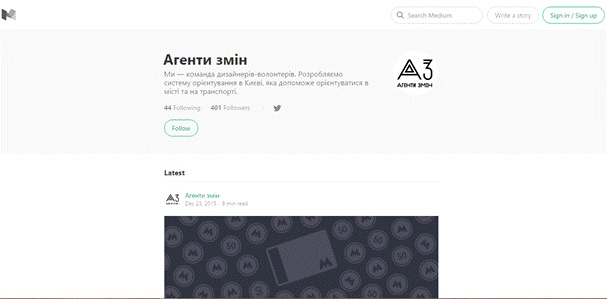
\includegraphics{images/022.jpg}

\subsection{Лун.UA}

\begin{itemize}
    \item \href{http://www.lun.ua/}{lun.ua} — оренда та продаж нерухомості у Києві та Україні.
\end{itemize}

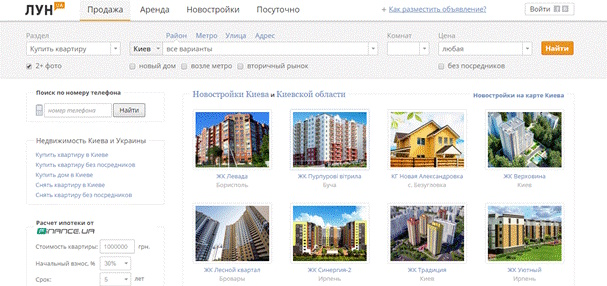
\includegraphics{images/023.jpg}

\subsection{PEP.ORG.UA}

\begin{itemize}
    \item \href{http://pep.org.ua/uk/}{pep.org.ua/uk/} — відкритий реєстр національних публічних діячів України.
\end{itemize}

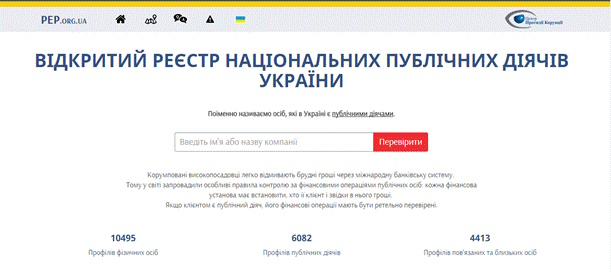
\includegraphics{images/024.jpg}

\subsection{Посіпаки}

\begin{itemize}
    \item \href{http://posipaky.info/}{posipaky.info} — база даних помічників народних депутатів України.
\end{itemize}

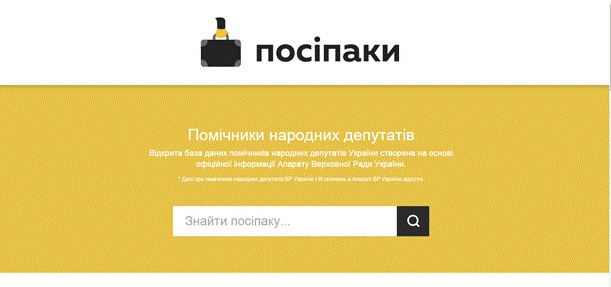
\includegraphics{images/025.jpg}

\subsection{CityScale}

\begin{itemize}
    \item \href{http://www.cityscale.com.ua/}{cityscale.com.ua} — портал з інтерактивними картами умов життя.
\end{itemize}

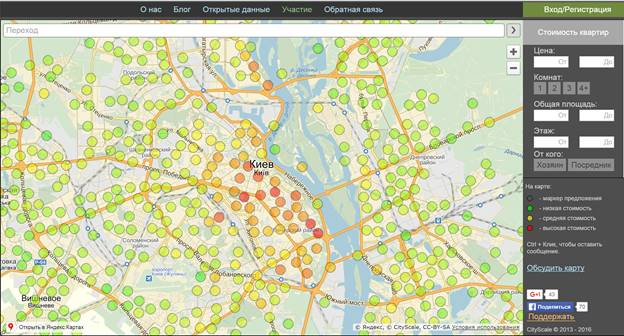
\includegraphics{images/026.jpg}

\subsection{ARBUZ}

Мобільний додаток для підвищення безпеки у містах на основі офіційних даних поліції.

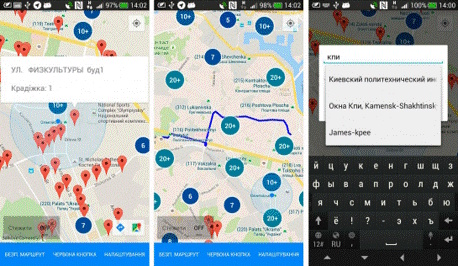
\includegraphics{images/027.jpg}

\subsection{KyivSmartCity}

\begin{itemize}
    \item \href{http://re.kievcity.gov.ua/#/objects}{re.kievcity.gov.ua/#/objects} — система управління майном громади Києва.
\end{itemize}

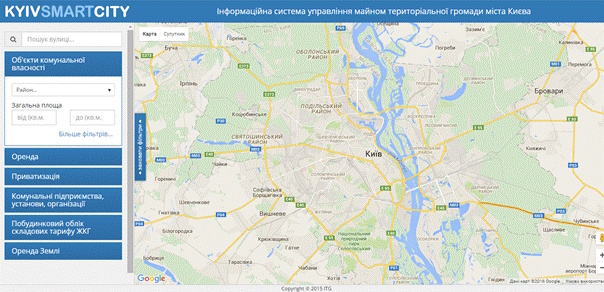
\includegraphics{images/028.jpg}

\subsection{Видані направлення авіакомпаніям України}

\begin{itemize}
    \item \href{https://www.google.com/maps/d/viewer?mid=zQyzchol-IlQ.kqJvVjvXIY-s&hl=en_US}{Google Maps} — призначення для експлуатації міжнародних повітряних ліній.
\end{itemize}

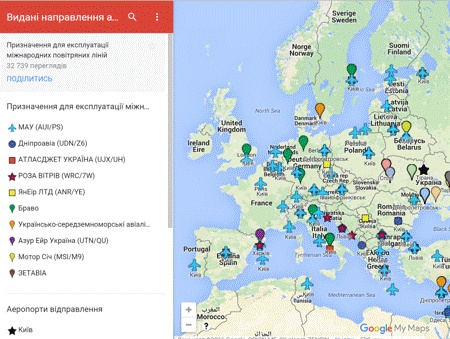
\includegraphics{images/029.jpg}

\subsection{Tesla Club Ukraine}

\begin{itemize}
    \item \href{http://tesla-club.com.ua/gmap}{tesla-club.com.ua/gmap} — мережа заправок для електромобілів.
\end{itemize}

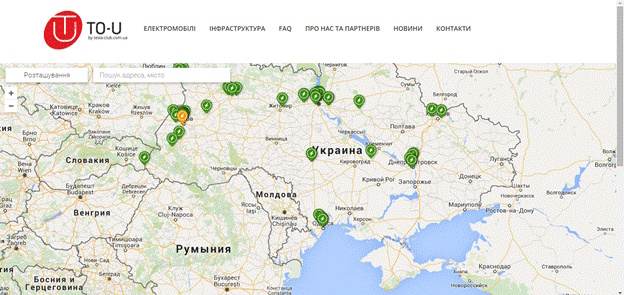
\includegraphics{images/030.jpg}

\subsection{Дороги України}

\begin{itemize}
    \item \href{http://uaroads.com/}{uaroads.com} — інформація про стан доріг в Україні.
\end{itemize}

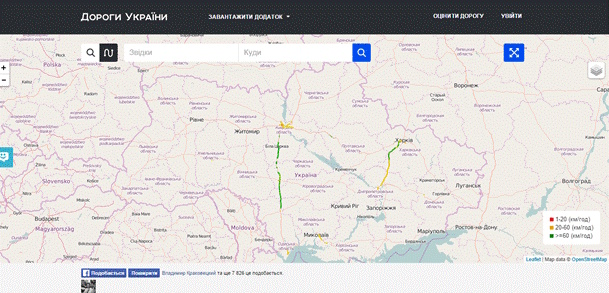
\includegraphics{images/031.jpg}

\subsection{Інші проєкти}

\begin{enumerate}
    \item \href{http://data.rada.gov.ua/open/main/apps}{Додатки та сервіси на базі відкритих даних ВРУ}
    \item \href{http://opendata.rada.gov.ua/}{Портал відкритих даних ВРУ}
    \item \href{http://rada4you.org}{Як голосують депутати}
    \item Мобільний додаток «Zakonoproekt» для відстеження законопроєктів
    \item \href{http://knopkodavy.chesno.org/}{Кнопкодави}
    \item \href{http://groups.chesno.org/}{Візуалізація даних спільного ініціювання законопроєктів}
    \item \href{https://rada.oporaua.org/map/}{Приймальні депутатів}, \href{https://pryjmalni.chesno.org}{pryjmalni.chesno.org}
    \item \href{http://openvote.in.ua/}{Виборча варта}
    \item \href{https://e-vybory.org/}{Електронні вибори}
\end{enumerate}

\subsection{Інкубатор на базі відкритих даних 1991}

1991 — перший в Україні некомерційний інкубатор, що допомагає перетворити відкриті державні дані на стартапи для громадян, бізнесу та держави.

Програми інкубатора:
\begin{itemize}
    \item Галузеві рішення (інфраструктура, агро, енергетика)
    \item Електронні послуги (для населення, у т.ч. на умовах ДПП)
    \item Аналітичні системи (для міністерств і органів влади)
    \item Smart-City рішення (для місцевих адміністрацій)
\end{itemize}

\chapter{Ресурси}
\label{sec:references}

\begin{enumerate}
    \item \textbf{visualizing.org} \\
    \url{http://www.visualizing.org} \\
    Спільнота і інформаційна платформа про візуалізації даних.

    \item \textbf{Google Chart Tools} \\
    \url{http://code.google.com/apis/chart/} \\
    Javascript API від Google для простого створення таблиць візуалізації для постійно змінюються даних.

    \item \textbf{GeoCommons} \\
    \url{http://geocommons.com} \\
    Інструментарій, спільнота і сервіс візуалізації для спільного використання геоданих.

    \item \textbf{Quadrigram} \\
    \url{http://www.quadrigram.com} \\
    Професійна платформа з можливістю платного побудови кастомізованих візуалізацій.

    \item \textbf{JavaScript InfoVis Toolkit} \\
    \url{http://thejit.org} \\
    Javascript-інструментарій для створення і підтримки візуалізації різного роду графіків.

    \item \textbf{d3.js - Data-Driven Documents} \\
    \url{http://mbostock.github.com/d3/} \\
    Маленька і дуже гнучка JavaScript бібліотека з відкритим вихідним кодом для управління документами на основі даних (наприклад, для генерації HTML5 або SVG-діаграми з даних).

    \item \textbf{Google Public Data Explorer} \\
    \url{http://www.google.com/publicdata/home} \\
    Каталог загального набору даних та інструмент для публікації і візуалізації великих наборів даних.

    \item \textbf{Maps Marker WP-Plugin} \\
    \url{http://www.mapsmarker.com} \\
    Wordpress-плагін для відображення карти з анотацією видатних пам'яток в блозі Wordpress.

    \item \textbf{DataMaps.eu - map your data} \\
    \url{http://www.datamaps.eu/} \\
    Інструмент для створення привабливих карт візуалізації, які можуть бути створені в браузері через веб-сайт без знання програмування.

    \item \textbf{Ushahidi} \\
    \url{http://www.ushahidi.com} \\
    Відкрите програмне забезпечення для збору, візуалізації та інтерактивного відображення на основі визначення місця розташування даних в реальному часі (наприклад, від надзвичайних ситуацій, політичних виборів і т.д.).

    \item \textbf{Eclipse BIRT} \\
    \url{http://www.eclipse.org/birt/phoenix/} \\
    Система звітності eclipse для створення візуально привабливих звітів великих обсягів даних.

    \item \textbf{Chartle.net} \\
    \url{http://www.chartle.net} \\
    Безкоштовне інтерактивний онлайн-додаток по створенню графіків. Інтуїтивно зрозумілий інтерфейс, не вимагає спеціальних навичок, проте і набір можливостей обмежений. Застосовується, коли потрібен швидкий результат: круглі і стовпчасті діаграми, лінійні графіки, динамічні схеми, географічна карта двох видів. Підсумкова візуалізація інтерактивна, і її код легко вбудовується в html-сторінку.

    \item \textbf{Hohli} \\
    \url{http://charts.hohli.com/} \\
    Простий і скромний інтерактивний безкоштовний онлайн-інструмент для візуалізації даних за допомогою стандартного набору діаграм. (Немає можливості створювати карти.)

    \item \textbf{IBM Many Eyes} \\
    \url{http://www-958.ibm.com/software/data/cognos/manyeyes/} \\
    Популярний онлайн-інструмент для візуалізації даних. Безкоштовний. Є можливість спільної роботи над проектами.

    \item \textbf{TagCrowd} \\
    \url{http://www.tagcrowd.com} \\
    Онлайн-додаток для аналізу і візуалізації частотності вживання слів у тексті. Безкоштовний.

    \item \textbf{Wordle} \\
    \url{http://www.wordle.net} \\
    Онлайн-додаток для аналізу і візуалізації частотності вживання слів у тексті. Безкоштовний.

    \item \textbf{Tableau} \\
    \url{http://www.tableausoftware.com} \\
    Сімейство програм для візуалізації даних. Асортимент опцій для кастомізації, а також можливість комбінувати кілька візуалізацій на одній панелі. За підсумками створення візуалізації можна отримати html-код, який можна вбудувати в веб-сторінку. Графіки інтерактивні. Закритий софт, однак, є безкоштовна версія з великою кількістю доступних можливостей (Tableau Public).

    \item \textbf{Dundas} \\
    \url{http://www.dundas.com} \\
    Програмне забезпечення для створення інтерактивних візуалізацій. Може обробляти великі масиви даних. Створює візуалізації, в числі іншого, у вигляді панелей з декількох компонентів, що дозволяє одночасно представити кілька вимірів. Працює онлайн, комерційне, платне. Пропонують 45-денний безкоштовний випробувальний термін.

    \item \textbf{Leximancer} \\
    \url{https://www.leximancer.com} \\
    Професійна програма для аналізу тексту та візуалізації результатів цього аналізу. Комерційна, платна, кроссплатформенная.

    \item \textbf{SIMILE Widgets} \\
    \url{http://www.simile-widgets.org} \\
    Збірка різноманітних віджетів і їх кодів. Коди відкриті з можливістю адаптувати під свої потреби, але для цього потрібні відповідні навички. Серед іншого, є інструменти, що дозволяють обробляти великі масиви даних і конструювати карти, тайм-лайни, інтерактивні таблиці і багато іншого. Інструмент Exibit дозволяє створювати цілі інтерактивні веб-сторінки з можливістю пошуку і самостійного дослідження представленої бази даних.

    \item \textbf{GeoCommons} \\
    \url{http://geocommons.com} \\
    Безкоштовний веб-інструмент зі створення карт на основі даних.

    \item \textbf{Gephi} \\
    \url{http://gephi.org} \\
    Програмне забезпечення для візуалізації графів. Використовується як один з інструментів аналізу соцмереж. Безкоштовний, відкритий код, кроссплатформлений.

    \item \textbf{Graphviz} \\
    \url{http://www.graphviz.org} \\
    Програма для візуалізації графів. Відкритий код, кросплатформенна, безкоштовна.

    \item \textbf{NewRadial} \\
    \url{http://sourceforge.net/projects/newradial/} \\
    Комплекс інструментів для візуального представлення нечислових даних (в тому числі зображень).

    \item \textbf{Prefuse} \\
    \url{http://www.prefuse.org} \\
    Великий набір різних інструментів для створення складних інтерактивних візуалізацій. Вимагають вміння програмувати. Безкоштовний, код відкритий.

    \item \textbf{ТЕКСТИ.ORG.UA} \\
    \url{http://texty.org.ua/pg/blog/infoviz} \\
    Блог: Інфовіз: інфографіка, інтерактивна візуалізація даних.

    \item \textbf{Charted} \\
    \url{http://www.charted.co/} \\
    Швидка візуалізація CSV файлів.

    \item \textbf{Venngage} \\
    \url{https://venngage.com/} \\
    Комерційний сервіс для створення інфографіки.

    \item \textbf{Dipity} \\
    \url{http://www.dipity.com/} \\
    Створення гарних таймлайнів.

    \item \textbf{Easily} \\
    \url{https://piktochart.com/} \\
    Генератор інфографіки.

    \item \textbf{Automatic Infographic Generator} \\
    \url{http://petercv.com/aig/} \\
    Генератор інфографіки.
\end{enumerate}
\chapter{Глосарій}
\label{sec:glossary}

\subsection{Додаток 2. Глосарій}
\begin{description}
\item[Абстрактна модель] — модель, що відображає загальні характеристики явища. Вона представляє інформацію про якісні характеристики об'єкта чи явища.
\item[Відкрита ліцензія] — документ, що визначає права й обмеження щодо об'єкта, регламентує вільне поширення контенту та/або програмного забезпечення. Свобода означає можливість використання, аналогічну свободі слова.
\item[Відкриті дані (Open Data)] — систематизована інформація, доступна через Інтернет у форматі, що дозволяє автоматизовану обробку, вільний і безоплатний доступ, а також подальше використання.
\item[Відкриті державні дані (Open Government Data)] — публічна інформація у вигляді відкритих даних про діяльність органів влади або створена в результаті їх діяльності.
\item[Власник інформації] — особа, яка створила інформацію або отримала право дозволяти чи обмежувати доступ до неї на підставі закону чи договору.
\item[Ідентифікатор набору відкритих даних (URN, Uniform Resource Name)] — постійний строковий параметр у визначеному форматі для ідентифікації та формування назв файлів набору, що включає інформацію про орган-власник, систему, тип даних, дати публікації й оновлення тощо.
\item[Інтерфейс прикладного програмування (API, Application Programming Interface)] — набір класів, функцій, структур і констант, доступних як сервіси через Інтернет для використання у прикладних програмах.
\item[Машинозчитувані дані] — дані у форматах, придатних для автоматичного використання.
\item[Метадані (метаінформація)] — структуровані дані, що визначають характеристики відкритих даних для їх ідентифікації та обробки.
\item[Набір відкритих даних (набір даних)] — сукупність однорідних записів, що містять структуровану інформацію — поля даних і метаінформацію.
\end{description}

\chapter{Посилання та література}
\label{sec:links-and-literature}

% Content from 07-links-and-literature.md
\subsection{Посилання та література}
\begin{enumerate}
\item \href{https://www.youtube.com/watch?v=nR9CXA6_7-I}{Відео. Як поєднати технології і волонтерський рух? | Дмитро Чаплинський | TEDxKPI}
\item \href{http://www.epravda.com.ua/publications/2015/08/20/554624}{Оцифровування статистики, або Перша їжа для Bigdata}
\item \href{http://platfor.ma/magazine/text-sq/projects/open-data-incubator/}{Данные нам: какие полезные сервисы Украина может получить от огромного массива своей информации}
\item \href{http://itc.ua/articles/bezopasnost-kak-usluga-uroki-parizhskih-teraktov-dlya-ukrainskih-operatorov}{Безопасность как услуга: уроки парижских терактов для украинских операторов}
\item \href{http://theodi.org/blog/ukraine-embracing-open-data-2014-revolution}{How Ukraine is embracing open data after the 2014 revolution}
\item \href{https://www.youtube.com/watch?v=gyHEOpX1yes}{Відкриті дані в Україні: що і як маємо відкрити? УКМЦ-04-03-2016}
\item \href{https://habrahabr.ru/post/306414/}{О развитии сферы открытых данных в Украине}
\end{enumerate}

\end{document}